% !TEX program = tectonic
\documentclass[10pt,a4paper,twocolumn]{article}
\usepackage{iftex}
\ifPDFTeX
  \usepackage[T1]{fontenc}
  \usepackage{lmodern}
  \usepackage[utf8]{inputenc}
\else
  \usepackage{fontspec}        % XeTeX/LuaTeX (tectonic) : UTF-8 natif
\fi
\usepackage[french]{babel}
\frenchsetup{StandardLists=true}
\usepackage[a4paper,margin=1.5cm,columnsep=0.6cm,footskip=0.7cm]{geometry}
\usepackage{amsmath,amssymb}
\usepackage{booktabs}
\usepackage{array}
\usepackage{graphicx}
\usepackage{enumitem}
\setlist[itemize]{leftmargin=1.1em,itemsep=0.5pt,topsep=1.5pt,parsep=0pt}
\setlist[enumerate]{leftmargin=1.5em,itemsep=0.5pt,topsep=1.5pt,parsep=0pt}
\usepackage{xcolor}
\usepackage[font=small,skip=2pt]{caption}
\usepackage{titlesec}
\titlespacing{\section}{0pt}{0.7em}{0.25em}
\titleformat{\section}{\normalsize\bfseries}{\thesection.}{0.4em}{}
\usepackage{hyperref}
\hypersetup{colorlinks=true,linkcolor=blue!50!black,urlcolor=blue!50!black}
\setlength{\parindent}{0pt}
\setlength{\parskip}{0.25em}
\raggedbottom
\setlength{\emergencystretch}{1.5em}
\abovedisplayskip=3pt plus 1pt \belowdisplayskip=3pt plus 1pt
\abovedisplayshortskip=2pt \belowdisplayshortskip=2pt
\newcommand{\code}[1]{\texttt{\small #1}}

\title{\vspace{-1.8em}\textbf{Le portefeuille de chaque élu du Congrès bat-il le marché ?}\\[2pt]
\large Classement par Information Ratio, ajustement au marché ($\beta$) et stratégie de copie corrigée (2014--2026)\\[1pt]
\small Note de synthèse --- \code{05b\_Portefeuille\_Membre\_MathSpec.ipynb}}
\author{\small Alice Lemaire --- 6 juillet 2026}
\date{\vspace{-2.6em}}

\begin{document}
\maketitle

\section{L'essentiel}
\begin{itemize}
  \item On reconstruit le portefeuille de \textbf{chaque membre} du Congrès à partir de ses transactions
        déclarées, on le compare au SPY, on classe, puis on teste la copie des meilleurs --- désormais avec
        l'\textbf{ajustement au marché} ($\beta$) et la \textbf{combinaison buy-and-hold corrigée}.
  \item Classement : \textbf{266 classés} $\to$ \textbf{223 éligibles} $\to$ \textbf{20 « significatifs »}
        par l'IR\dots{} mais \textbf{12} par l'appraisal ($\beta$ retiré) $\approx$ \textbf{$\sim$11 attendus
        par pur hasard} sur 223 tests : le surnombre était du $\beta$.
  \item En \textbf{walk-forward}, la tête du classement change presque chaque année ;
        seules \textbf{S.~DelBene} et \textbf{B.~Comstock} sont robustes.
  \item Stratégie \textbf{top-4 corrigée} (2016--2026) : $+3{,}1\,\%$/an vs SPY, $t=0{,}94 <$
        seuil $\approx 1{,}81$. L'ancienne combinaison à poids figés ($+3{,}6\,\%$, $t=1{,}14$)
        rebalançait chaque jour et \textbf{flattait} le résultat.
  \item $\beta \approx 1{,}20 \Rightarrow \alpha = -0{,}4\,\%$/an ($t_{\text{appr}}=-0{,}13$) :
        l'excès n'est que de l'\textbf{exposition au marché}. Pas d'alpha, même en plafond théorique
        (entrée à la transaction, sans frais ; la version jouable est le notebook~06).
  \item \textbf{Aucun $K$ de 4 à 20 ne sauve la stratégie} --- même en laissant le $K$ se choisir
        chaque année en walk-forward ($t=1{,}58<1{,}81$, $t_{\text{appr}}=0{,}45$).
\end{itemize}

\section{Données}
\begin{itemize}
  \item Transactions : table canonique S1/S2\\
        \code{transactions\_backtest\_2014\_2026.csv},\\
        $134\,464 \to 134\,429$ lignes, \textbf{372 membres}, $4\,618$ tickers ;
        actions + ETF, nettoyage transactionnel fait en amont.
  \item Dates \emph{déclarées} 2014--2026 ; la date d'\emph{opération} (\code{traded})
        remonte parfois à 2013 (déclaration à retardement, STOCK Act) --- seules les
        35 opérations de 2012 sont écartées.
  \item Panel de prix (cache \code{prices\_v2}, Yahoo) : $3\,289$ tickers avec prix,
        $1\,268$ sans prix, \textbf{61 corrompus exclus} $\to$ $16\,400$ trades jetés,
        $\mathbf{118\,029}$ exploitables. Le SPY donne le calendrier de bourse maître.
\end{itemize}

\section{Méthode}
Notations : $i$ = ticker, $t$ = jour de bourse, $P_i(t)$ = cours de clôture.

\textbf{(a) Reconstruction du portefeuille.} Achat $\to$ parts au 1\ier{} jour coté
$\ge$ la transaction ; vente $\to$ retire des parts (short interdit) ; détentions cumulées :
$$q = \frac{\text{montant}}{P_i(\tau)},\qquad \tau=\min\{t \ge \code{traded}\}$$
$$q^- = \min\!\Big(\tfrac{\text{montant}}{P_i},\, \text{parts}\Big),\;\;
  n_i(t) = \!\!\sum_{\text{achats}\le t}\! q \,-\!\! \sum_{\text{ventes}\le t}\! q^-$$
et $V(t)=\sum_i n_i(t)\,P_i(t)$.

\textbf{(b) Rendement \emph{time-weighted}.} On valorise les parts de la \emph{veille}
(un apport n'est jamais un rendement) :
$$r_P(t) = \frac{\sum_i n_i(t-1)\,P_i(t)}{\sum_i n_i(t-1)\,P_i(t-1)} - 1$$
Jour sans position : $r_P=0$ (système ouvert) ; winsorisation $\pm 50\,\%$/jour.
$\mathrm{NAV}(t)=\prod_{s\le t}(1+r_P(s))$, $\mathrm{vol}=\sigma(r_P)\sqrt{252}$,
$\mathrm{Sharpe}=\tfrac{\overline{r_P}}{\sigma(r_P)}\sqrt{252}$.

\textbf{(c) Excès et Information Ratio.} $r_{SPY}(t)=\tfrac{SPY(t)}{SPY(t-1)}-1$,
$x(t)=r_P(t)-r_{SPY}(t)$ :
$$\mathrm{IR}=\frac{\overline{x}}{\sigma(x)}\sqrt{252},\qquad
  t=\mathrm{IR}\sqrt{\tfrac{n}{252}}>1{,}645$$

\textbf{(d) Ajustement par le marché.} L'IR soustrait \emph{tout} le SPY $\Rightarrow$ il suppose
$\beta=1$ ; un portefeuille agressif affiche un excès positif en marché haussier \emph{sans talent}.
On régresse les rendements quotidiens :
$$r_P(t)=\alpha+\beta\,r_{SPY}(t)+\varepsilon(t)$$
$$\beta=\frac{\operatorname{Cov}(r_P,r_{SPY})}{\operatorname{Var}(r_{SPY})},\qquad
  \alpha=\overline{r_P}-\beta\,\overline{r_{SPY}}$$
$\beta$ = exposition (levier de \emph{style}), $\alpha$ = le \emph{talent}. L'\textbf{appraisal}
= l'IR du résidu $\varepsilon$, avec son test (même construction, seuil identique) :
$$\text{appraisal}=\frac{\alpha}{\sigma(\varepsilon)}\sqrt{252},\;\;
  t_{\text{appr}}=\text{appraisal}\sqrt{\tfrac{n}{252}}>1{,}645$$
$\beta=1 \Rightarrow$ appraisal $=$ IR ; sinon l'IR mélange exposition et talent.

\textbf{Illustration sur un membre : B.~Comstock} --- un \emph{bon} exemple : 85 trades
sur 2\,390 jours, portefeuille diversifié (44 tickers déclarés, AAPL n'en fait que 10),
robuste au walk-forward et significative \emph{aux deux tests}. $V(t)$ saute à chaque trade
(apports + performance mélangés) ; la NAV isole la performance pure ; la régression donne
son $\beta$ et son talent : IR 0,90 ($t$ 2,77), $\beta$ 1,20, $\alpha_{\text{ann}}$ $+7{,}5\,\%$,
appraisal 0,66 ($t_{\text{appr}}$ 2,03) ; CAGR $+26{,}2\,\%$, vol 25\,\%, maxDD $-33\,\%$.
\emph{NB : filtre par \code{bioguide\_id} et non par nom --- certains élus portent plusieurs
variantes de nom dans les dépôts (Comstock en a deux).}

\begin{center}
\begin{minipage}{\linewidth}\centering
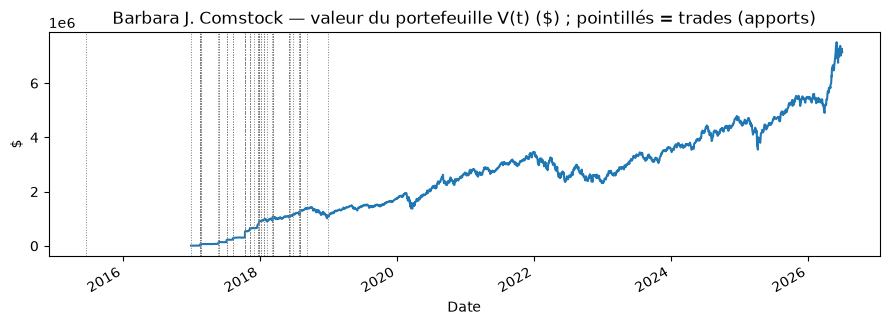
\includegraphics[width=\linewidth]{figures/fig_nb05b_vt_membre.png}
\captionof{figure}{$V(t)$ du membre démo --- chaque pointillé est un trade : la \emph{valeur}
mélange apports et performance.}
\end{minipage}
\end{center}

\begin{center}
\begin{minipage}{\linewidth}\centering
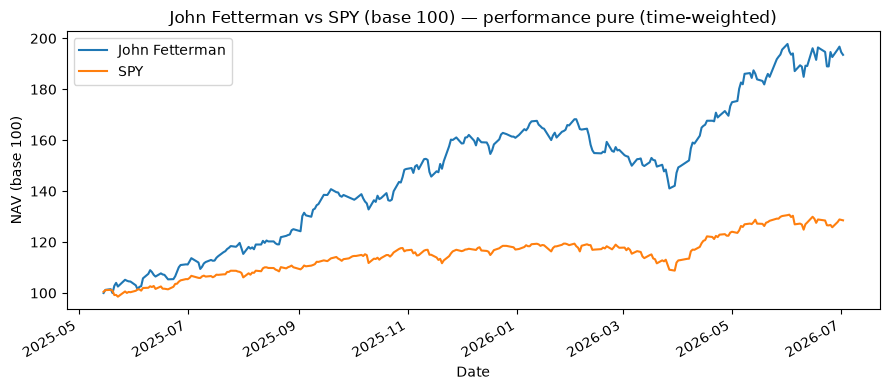
\includegraphics[width=\linewidth]{figures/fig_nb05b_nav_membre.png}
\captionof{figure}{La NAV (base 100) du même membre vs SPY : performance pure, débarrassée
des apports (\emph{time-weighted}).}
\end{minipage}
\end{center}

\begin{center}
\begin{minipage}{\linewidth}\centering
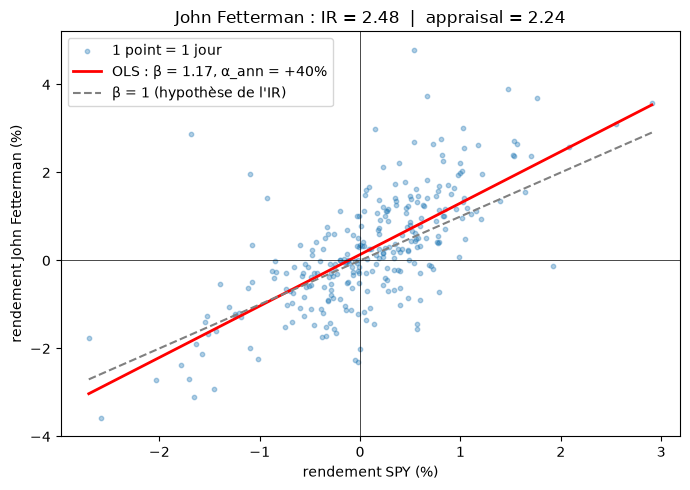
\includegraphics[width=0.8\linewidth]{figures/fig_nb05b_reg_membre.png}
\captionof{figure}{La régression du membre démo : 1 point $=$ 1 jour ; pente $=\beta=1{,}20$,
ordonnée $=\alpha$ ; la droite grise est l'hypothèse $\beta=1$ de l'IR.}
\end{minipage}
\end{center}

\section{Classement : IR vs appraisal}
\begin{itemize}
  \item \textbf{Éligibilité} : $\ge 10$ trades et $\ge 126$ jours ($\sim$6 mois) $\Rightarrow$
        $266 \to 223$ membres. Sur 223 tests à 5\,\%, $\sim$11 « significatifs » sont attendus
        par pur hasard.
  \item Par l'\textbf{IR} : \textbf{20} membres à $t>1{,}645$. Par l'\textbf{appraisal} :
        \textbf{12} à $t_{\text{appr}}>1{,}645$ --- retour \textbf{au niveau du hasard} :
        la queue droite « significative » était surtout du $\beta$.
  \item Les portés par le marché \textbf{chutent} : Moody ($\beta=1{,}79$) passe de $t=2{,}01$
        à $t_{\text{appr}}=1{,}64$ (sous le seuil), Lawrence ($\beta=1{,}50$) de 2,24 à 1,34.
        Des défensifs \textbf{montent} : Ruiz ($\beta=0{,}09$, IR $-0{,}05$) devient n°1 du
        test appraisal ($t_{\text{appr}}=2{,}40$).
  \item \textbf{Biais petits échantillons} toujours là : Fetterman, n°1 des deux classements
        (IR 2,48, appraisal 2,24), ne repose que sur \textbf{10 trades / 284 jours}.
\end{itemize}

\begin{center}
\begin{minipage}{\linewidth}\centering\footnotesize\setlength{\tabcolsep}{3pt}
\begin{tabular}{lrrrrrrr}
\toprule
\textbf{Membre} & \textbf{trades} & \textbf{jours} & \textbf{IR} & $\boldsymbol{t}$ & $\boldsymbol{\beta}$ & \textbf{appr.} & $\boldsymbol{t_{\text{appr}}}$\\
\midrule
Comstock  &  85 & 2\,390 & 0,90 & 2,77 & 1,20 & 0,66 & 2,03\\
McGarvey  &  24 &   853 & 1,50 & 2,76 & 1,53 & 1,08 & 1,99\\
Suozzi    & 662 & 2\,230 & 0,90 & 2,68 & 1,22 & 0,59 & 1,75\\
Fetterman &  10 &   284 & 2,48 & 2,64 & 1,17 & 2,24 & 2,38\\
DelBene   & 157 & 3\,054 & 0,66 & 2,30 & 1,15 & 0,52 & 1,81\\
Lawrence  &  19 & 2\,430 & 0,72 & 2,24 & 1,50 & 0,43 & 1,34\\
Warner    &  15 & 1\,934 & 0,80 & 2,22 & 1,78 & 0,65 & 1,80\\
Babin     &  20 & 2\,573 & 0,69 & 2,21 & 1,18 & 0,62 & 1,99\\
\bottomrule
\end{tabular}
\captionof{table}{Top-8 par $t$ (test IR), avec nombre de trades, jours de track, $\beta$ et test appraisal en regard.}
\end{minipage}
\end{center}

\begin{center}
\begin{minipage}{\linewidth}\centering\footnotesize\setlength{\tabcolsep}{3pt}
\begin{tabular}{lrrrrrrr}
\toprule
\textbf{Membre} & \textbf{trades} & \textbf{jours} & \textbf{IR} & $\boldsymbol{t}$ & $\boldsymbol{\beta}$ & \textbf{appr.} & $\boldsymbol{t_{\text{appr}}}$\\
\midrule
Ruiz          &  10 & 2\,261 & $-$0,05 & $-$0,16 & 0,09 & 0,80 & 2,40\\
Fetterman     &  10 &   284 & 2,48 & 2,64 & 1,17 & 2,24 & 2,38\\
Comstock      &  85 & 2\,390 & 0,90 & 2,77 & 1,20 & 0,66 & 2,03\\
Sessions      & 361 & 3\,376 & 0,31 & 1,15 & 0,93 & 0,55 & 2,01\\
Babin         &  20 & 2\,573 & 0,69 & 2,21 & 1,18 & 0,62 & 1,99\\
McGarvey      &  24 &   853 & 1,50 & 2,76 & 1,53 & 1,08 & 1,99\\
Hollingsworth &  18 & 1\,494 & 0,21 & 0,52 & 0,43 & 0,79 & 1,92\\
Whitehouse    & 718 & 3\,316 & 0,57 & 2,07 & 1,04 & 0,51 & 1,85\\
\bottomrule
\end{tabular}
\captionof{table}{Top-8 par $t_{\text{appr}}$ (test appraisal) : des profils \emph{défensifs}
(Ruiz, Hollingsworth) apparaissent, invisibles au test IR.}
\end{minipage}
\end{center}

\begin{center}
\begin{minipage}{\linewidth}\centering
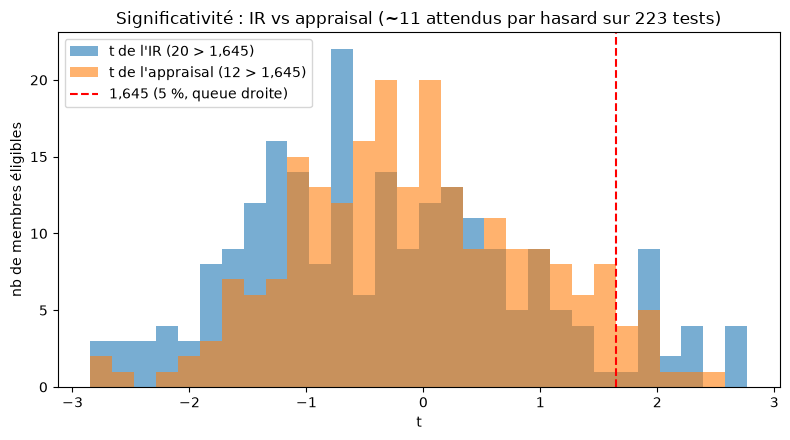
\includegraphics[width=0.92\linewidth]{figures/fig_nb05b_hist_2t.png}
\captionof{figure}{Distribution des deux $t$ sur les 223 éligibles : retirer le $\beta$ dégonfle
la queue droite (20 $\to$ 12 $\approx$ hasard).}
\end{minipage}
\end{center}

\begin{center}
\begin{minipage}{\linewidth}\centering
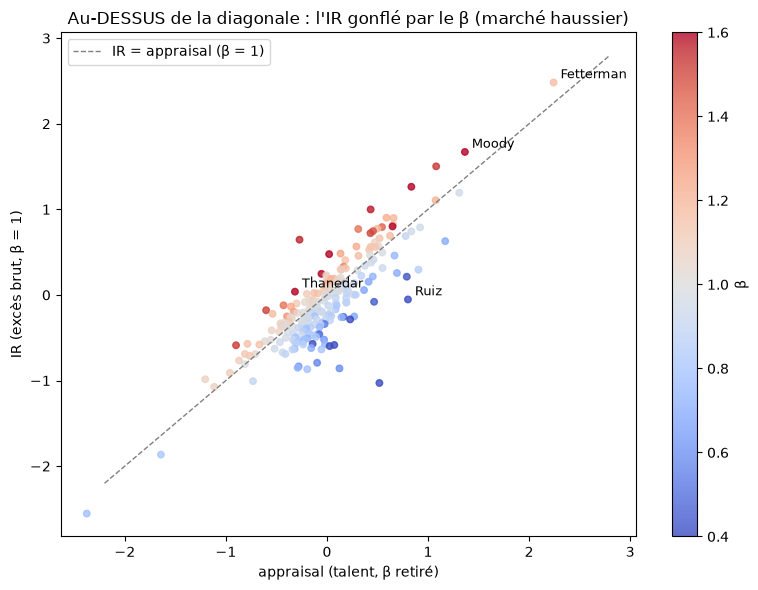
\includegraphics[width=0.85\linewidth]{figures/fig_nb05b_scatter_ir_appr.png}
\captionof{figure}{IR vs appraisal, couleur $=\beta$ : au-dessus de la diagonale, l'IR
\emph{flattait} le membre (rouge $=$ haut $\beta$) ; en dessous, il le pénalisait (bleu $=$ défensif).}
\end{minipage}
\end{center}

\begin{center}
\begin{minipage}{\linewidth}\centering\footnotesize\setlength{\tabcolsep}{3.5pt}
\begin{tabular}{lrrrc}
\toprule
\textbf{Membre} & \textbf{IR} & $\boldsymbol{\beta}$ & \textbf{appr.} & \textbf{rang IR$\to$appr.}\\
\midrule
\multicolumn{5}{l}{\emph{Plus grosses chutes (le $\beta$ gonflait l'IR)}}\\
Fields    & 0,65 & 1,56 & $-$0,27 & 22 $\to$ 168\\
Thanedar  & 0,04 & 2,47 & $-$0,32 & 80 $\to$ 177\\
Morrison  & $-$0,18 & 1,52 & $-$0,60 & 117 $\to$ 208\\
\midrule
\multicolumn{5}{l}{\emph{Plus grosses montées (talent masqué par l'IR)}}\\
Graham    & $-$1,03 & 0,09 & 0,52 & 220 $\to$ 25\\
McCormick & $-$0,86 & 0,58 & 0,12 & 215 $\to$ 71\\
Crist     & $-$0,58 & 0,27 & 0,07 & 197 $\to$ 84\\
\bottomrule
\end{tabular}
\captionof{table}{Le reclassement IR $\to$ appraisal : qui chute, qui monte (223 éligibles).}
\end{minipage}
\end{center}

\section{Walk-forward (sans regard futur)}
\begin{itemize}
  \item Classement rejoué \textbf{fin de chaque année $Y$} avec les seules données $\le Y$
        (sélection suivie en $Y{+}1$) --- $n_i(t)$ ne dépend que des trades $\le t$, tronquer
        ne triche jamais.
  \item \textbf{Le n°1 change presque chaque année} : 11 têtes différentes sur 13 fenêtres.
  \item \textbf{Robustes} : DelBene significative à \emph{chaque} fenêtre depuis 2018,
        Comstock à toutes sauf une depuis 2017.
  \item Fetterman et Moody (n°1--2 plein échantillon) n'apparaissent qu'à la \emph{toute
        dernière} fenêtre : jamais suivis en direct $\Rightarrow$ motive un \textbf{top-$K$}.
\end{itemize}

\begin{center}
\begin{minipage}{\linewidth}\centering\footnotesize\setlength{\tabcolsep}{4pt}
\begin{tabular}{lrll}
\toprule
\textbf{Fenêtre} & $\boldsymbol{n_{\text{sig}}}$ & \textbf{n°1} & \textbf{n°2}\\
\midrule
2014--2014 &  1 & Reed      & ---\\
2014--2015 &  4 & McKinley  & Davis\\
2014--2016 &  2 & Long      & King\\
2014--2017 &  4 & Comstock  & Long\\
2014--2018 &  5 & Heck      & Evans\\
2014--2019 &  8 & Evans     & Heck\\
2014--2020 & 19 & Beyer     & Cisneros\\
2014--2021 & 13 & Comstock  & Warner\\
2014--2022 &  7 & DelBene   & Comstock\\
2014--2023 & 12 & Landsman  & Sullivan\\
2014--2024 & 17 & McGarvey  & McClain\\
2014--2025 & 20 & McGarvey  & Sullivan\\
2014--2026 & 20 & Fetterman & Moody\\
\bottomrule
\end{tabular}
\captionof{table}{Walk-forward : nb de significatifs et tête du classement à chaque coupe.}
\end{minipage}
\end{center}

\section{Stratégie top-4 : la bonne combinaison}
\begin{itemize}
  \item Fin d'année $Y$ : les \textbf{4 meilleurs IR} parmi les significatifs point-in-time
        (repli si moins de 4) ; copie du panier en $Y{+}1$, poids initiaux
        $w_k=\tfrac1K$ ou $\tfrac{\mathrm{IR}_k}{\sum_j \mathrm{IR}_j}$.
  \item \textbf{Écueil} : $\sum_k w_k\,r_{m_k}$ à poids \emph{figés} = rebalancer chaque jour.
        « Copier et \emph{tenir} » laisse les poids \textbf{dériver} (buy-and-hold) :
        $$N(t)=\sum_k w_k\,\mathrm{NAV}_k(t),\qquad
          r_{\text{strat}}(t)=\frac{N(t)}{N(t-1)}-1$$
        avec les poids effectifs $w_k(t)=\tfrac{w_k\,\mathrm{NAV}_k(t-1)}{\sum_j w_j\,\mathrm{NAV}_j(t-1)}$,
        remis à $w_k$ à chaque re-sélection annuelle.
\end{itemize}

\begin{center}
\begin{minipage}{\linewidth}\centering\small\setlength{\tabcolsep}{5pt}
\begin{tabular}{lrrrl}
\toprule
 & \textbf{A (Apple)} & \textbf{B (Coca)} & \textbf{Total} & $\boldsymbol{r_{\text{strat}}}$\\
\midrule
jour 0 &  50 & 50 & 100 & ---\\
jour 1 & 100 & 50 & 150 & $+50{,}00\,\%$\\
jour 2 & 100 & 60 & 160 & $+6{,}67\,\%$\\
\bottomrule
\end{tabular}
\captionof{table}{L'exemple ($K{=}2$, $w=\tfrac12,\tfrac12$) : au jour 2, la moyenne figée donnerait
$\tfrac12\!\cdot\!0+\tfrac12\!\cdot\!20=10\,\%$ (faux) ; les poids ont dérivé à $\tfrac23,\tfrac13$
$\Rightarrow$ $6{,}67\,\%$.}
\end{minipage}
\end{center}

\begin{itemize}
  \item Évaluation \textbf{par année} : $n=11$ (2016--2026), seuil $t_{10}\approx 1{,}81$.
        La correction \textbf{abaisse} le résultat :
\end{itemize}

\begin{center}
\begin{minipage}{\linewidth}\centering\small\setlength{\tabcolsep}{4pt}
\begin{tabular}{lrrrr}
\toprule
\textbf{Combinaison} & \textbf{excès/an} & $\mathbf{IR_{ann}}$ & $\boldsymbol{t}$ & \textbf{gagn.}\\
\midrule
$1/K$ figé (ancien)      & $+3{,}6\,\%$ & 0,34 & 1,14 & 7/11\\
$1/K$ dérive (corrigé)   & $\mathbf{+3{,}1\,\%}$ & 0,28 & \textbf{0,94} & 7/11\\
$\propto$IR figé         & $+3{,}5\,\%$ & 0,33 & 1,09 & 7/11\\
$\propto$IR dérive       & $+3{,}0\,\%$ & 0,27 & 0,90 & 7/11\\
\bottomrule
\end{tabular}
\captionof{table}{Stratégie top-4 vs SPY : ancienne combinaison vs corrigée.}
\end{minipage}
\end{center}

\begin{center}
\begin{minipage}{\linewidth}\centering
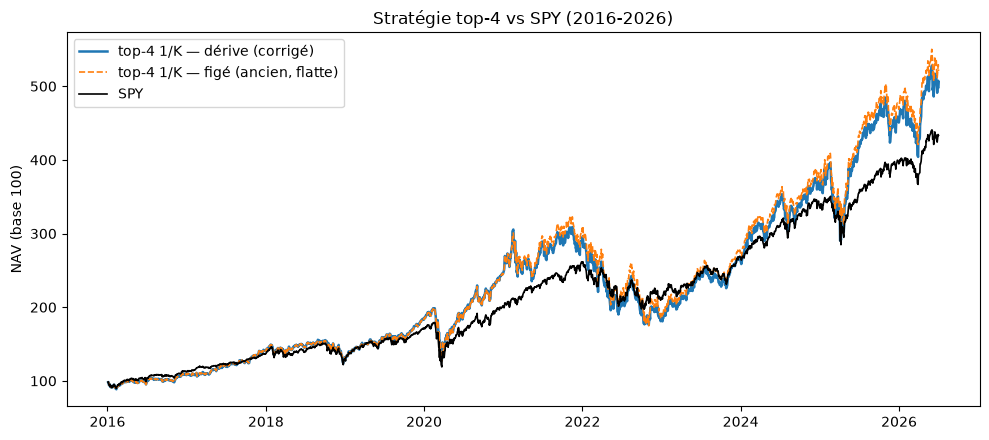
\includegraphics[width=\linewidth]{figures/fig_nb05b_nav_strat.png}
\captionof{figure}{NAV de la stratégie top-4 (corrigée et ancienne) vs SPY, base 100 (2016--2026).}
\end{minipage}
\end{center}

\begin{center}
\begin{minipage}{\linewidth}\centering
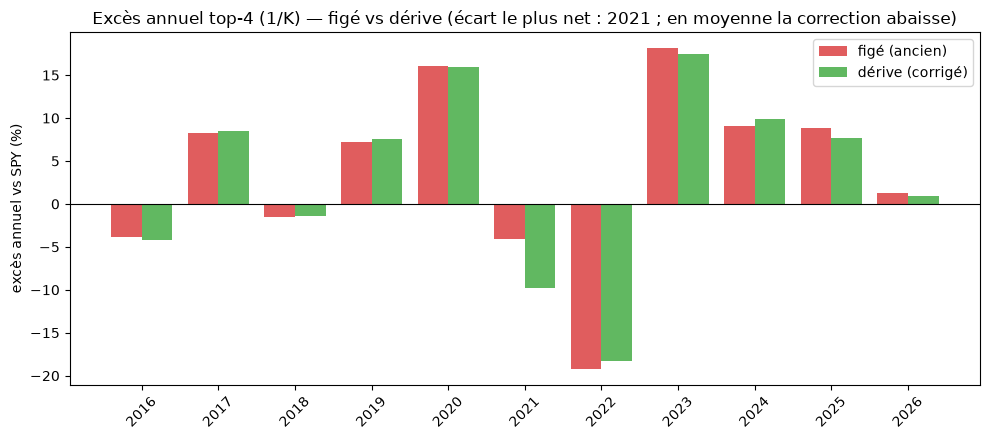
\includegraphics[width=0.92\linewidth]{figures/fig_nb05b_exces_fige_derive.png}
\captionof{figure}{Excès annuel top-4 ($1/K$) : combinaison figée vs corrigée (écart le plus net
en 2021 ; en moyenne la correction abaisse).}
\end{minipage}
\end{center}

\begin{itemize}
  \item \textbf{Ajustement au marché de la stratégie} (sur la série corrigée) :
\end{itemize}

\begin{center}
\begin{minipage}{\linewidth}\centering\small\setlength{\tabcolsep}{4pt}
\begin{tabular}{lrrrr}
\toprule
\textbf{Schéma} & $\boldsymbol{\beta}$ & $\boldsymbol{\alpha}_{\text{ann}}$ & \textbf{appr.} & $\boldsymbol{t_{\text{appr}}}$\\
\midrule
top-4 $1/K$        & 1,20 & $-0{,}4\,\%$ & $-0{,}04$ & $-0{,}13$\\
top-4 $\propto$IR  & 1,21 & $-0{,}6\,\%$ & $-0{,}06$ & $-0{,}19$\\
\bottomrule
\end{tabular}
\captionof{table}{$r_{\text{strat}}=\alpha+\beta\,r_{SPY}+\varepsilon$ : le $\beta$ porte tout, l'$\alpha$ est négatif.}
\end{minipage}
\end{center}

\begin{center}
\begin{minipage}{\linewidth}\centering
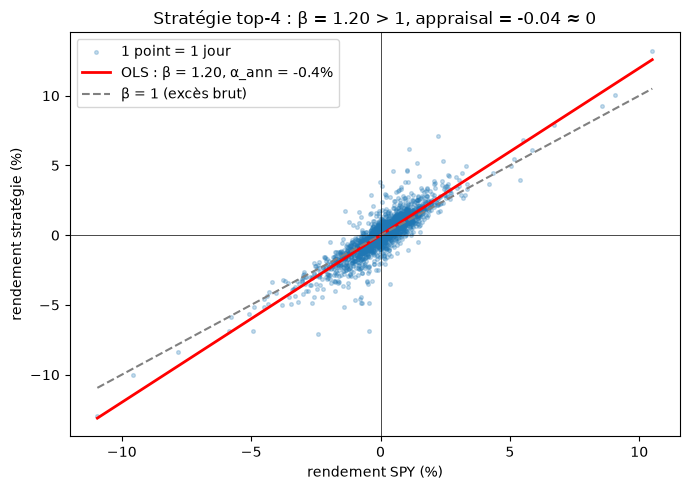
\includegraphics[width=0.8\linewidth]{figures/fig_nb05b_regression_strat.png}
\captionof{figure}{La régression de la stratégie : pente $\beta=1{,}20$ au-dessus de la droite
$\beta=1$ --- l'excès brut n'était que du marché amplifié.}
\end{minipage}
\end{center}

\section{Choisir $K$ : balayage et walk-forward}
\begin{itemize}
  \item $K=4$ était arbitraire ; on regarde $K \in [4, 20]$. Au-delà, le panier plafonne
        (rarement plus de $\sim$20 significatifs une année donnée ; si $n_{\text{sig}}(Y)<K$, repli).
  \item \textbf{Balayage statique} (diagnostic) : aucun $K$ ne franchit le seuil --- meilleur
        $t=1{,}74$ à $K{=}12$, et encore, choisi \emph{a posteriori} (regard futur).
  \item \textbf{Sélection honnête du $K$ (walk-forward)} : à fin $Y$,
        $$K^*(Y)=\arg\max_{K\in[4,20]}\ \mathrm{IR}_{\text{quotidien}}\big(\text{strat-}K\big|_{2016..Y}\big)$$
        (les séries strat-$K$ sont point-in-time, les tronquer ne regarde pas le futur ;
        fin 2015 : aucun historique $\to K^*{=}4$ par défaut). Panier de $K^*(Y)$ tenu en $Y{+}1$.
  \item Résultat : $+4{,}1\,\%$/an, $t=1{,}58<1{,}81$, $\alpha_{\text{ann}}=+1{,}1\,\%$
        ($t_{\text{appr}}=0{,}45$) --- \textbf{mieux que $K{=}4$ fixe, mais toujours pas d'alpha}.
\end{itemize}

\begin{center}
\begin{minipage}{\linewidth}\centering
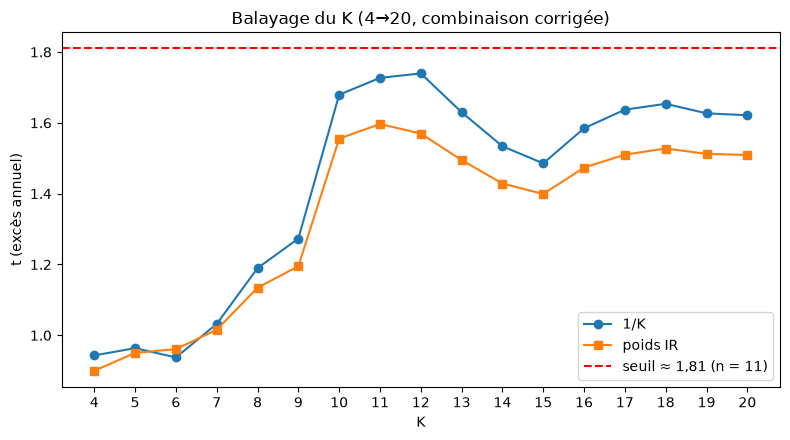
\includegraphics[width=0.88\linewidth]{figures/fig_nb05b_ksweep_t.png}
\captionof{figure}{Balayage du $K$ (combinaison corrigée) : le $t$ plafonne sous le seuil pour
tout $K$ de 4 à 20.}
\end{minipage}
\end{center}

\begin{center}
\begin{minipage}{\linewidth}\centering\footnotesize\setlength{\tabcolsep}{4pt}
\begin{tabular}{rrrrr}
\toprule
$\boldsymbol{K}$ & $\boldsymbol{n_{\text{moy}}}$ & \textbf{excès/an} & $\boldsymbol{t}$ & $\boldsymbol{t_{\text{appr}}}$\\
\midrule
 4 &  3,8 & $+3{,}1\,\%$ & 0,94 & $-$0,13\\
 6 &  5,2 & $+2{,}7\,\%$ & 0,94 & $-$0,15\\
 8 &  6,4 & $+3{,}4\,\%$ & 1,19 & 0,06\\
10 &  7,3 & $+5{,}0\,\%$ & 1,68 & 0,63\\
\textbf{12} &  8,2 & $+4{,}6\,\%$ & \textbf{1,74} & 0,66\\
14 &  8,8 & $+4{,}0\,\%$ & 1,53 & 0,47\\
16 &  9,4 & $+4{,}2\,\%$ & 1,59 & 0,55\\
18 &  9,8 & $+4{,}3\,\%$ & 1,65 & 0,65\\
20 & 10,1 & $+4{,}3\,\%$ & 1,62 & 0,62\\
\bottomrule
\end{tabular}
\captionof{table}{Balayage (schéma $1/K$, un $K$ sur deux) : $n_{\text{moy}}$ = taille réelle
moyenne du panier (repli). Bosse vers $K{=}10$--12, jamais au-dessus de 1,81.}
\end{minipage}
\end{center}

\begin{center}
\begin{minipage}{\linewidth}\centering\footnotesize\setlength{\tabcolsep}{4pt}
\begin{tabular}{rrrrr}
\toprule
\textbf{fin} $\boldsymbol{Y}$ & $\boldsymbol{K^*}$ & \textbf{IR passé} & \textbf{tenue} & \textbf{excès réalisé}\\
\midrule
2015 &  4 & ---     & 2016 & $-4{,}2\,\%$\\
2016 &  4 & $-$0,99 & 2017 & $+8{,}5\,\%$\\
2017 &  4 & 0,25    & 2018 & $-1{,}4\,\%$\\
2018 &  4 & 0,11    & 2019 & $+7{,}6\,\%$\\
2019 &  4 & 0,32    & 2020 & $+15{,}9\,\%$\\
2020 &  8 & 0,69    & 2021 & $-6{,}1\,\%$\\
2021 & 18 & 0,49    & 2022 & $-9{,}9\,\%$\\
2022 & 12 & 0,19    & 2023 & $+12{,}2\,\%$\\
2023 & 18 & 0,33    & 2024 & $+4{,}4\,\%$\\
2024 & 18 & 0,37    & 2025 & $+4{,}2\,\%$\\
2025 & 12 & 0,39    & 2026 & $+13{,}5\,\%$\\
\bottomrule
\end{tabular}
\captionof{table}{Le chemin du $K$ walk-forward (schéma $1/K$) : $K{=}4$ par défaut, puis le panier
grossit dès que l'historique montre que les grands $K$ font mieux.}
\end{minipage}
\end{center}

\begin{center}
\begin{minipage}{\linewidth}\centering\footnotesize\setlength{\tabcolsep}{2.8pt}
\begin{tabular}{lrrrrrr}
\toprule
\textbf{Stratégie} & \textbf{excès/an} & $\boldsymbol{t}$ & \textbf{gagn.} & $\boldsymbol{\beta}$ & $\boldsymbol{\alpha}_{\text{ann}}$ & $\boldsymbol{t_{\text{appr}}}$\\
\midrule
$K{=}4$ fixe ($1/K$)     & $+3{,}1\,\%$ & 0,94 & 7/11 & 1,20 & $-0{,}4\,\%$ & $-$0,13\\
$K$ w-f ($1/K$)          & $\mathbf{+4{,}1\,\%}$ & \textbf{1,58} & 7/11 & 1,17 & $+1{,}1\,\%$ & 0,45\\
$K{=}4$ fixe ($\propto$IR) & $+3{,}0\,\%$ & 0,90 & 7/11 & 1,21 & $-0{,}6\,\%$ & $-$0,19\\
$K$ w-f ($\propto$IR)    & $+3{,}6\,\%$ & 1,43 & 7/11 & 1,18 & $+0{,}6\,\%$ & 0,22\\
\bottomrule
\end{tabular}
\captionof{table}{$K$ fixe vs $K$ choisi en walk-forward : mieux, mais toujours sous le seuil,
et $\alpha \approx 0$ une fois le $\beta$ retiré.}
\end{minipage}
\end{center}

\section{Garde-fous, limites, verdict}
\textbf{Garde-fous décisifs} :
\begin{itemize}
  \item Filtre anti-corruption Yahoo : ticker exclu si prix min $<0{,}10\,\$$ ou saut
        journalier $>300\,\%$. \emph{Sans lui, un run précédent affichait $+12\,\%$/an d'excès
        factice, dû au seul glitch \code{DAIUF} (2022).}
  \item Winsorisation $r_P$ à $\pm 50\,\%$/jour ; flags amont S1/S2 (\code{is\_delisted} : 51 tickers).
\end{itemize}
\textbf{Limites honnêtes} :
\begin{itemize}
  \item \textbf{Survivorship} : univers $=$ tickers que Yahoo sert encore $\to$ bornes hautes.
  \item Entrée \code{traded} $=$ information parfaite ($\sim$1 mois d'avance sur un copieur réel) ;
        excès \textbf{brut}, sans coûts.
  \item $n=11$ années, très peu pour trancher ; seuils ad~hoc (10 trades / 126~j) ;
        $\sim$11 faux positifs attendus sur 223 tests.
\end{itemize}
\textbf{Verdict} : le classement est crédible et outillé, mais une fois l'exposition au marché
retirée, \textbf{il ne reste pas de talent mesurable} --- 12 « significatifs » $\approx$ hasard,
stratégie $\alpha<0$ (et $\alpha\approx 0$ même en laissant le $K$ se choisir tout seul).
À ne pas suivre en direct ; la version jouable (entrée à la publication + coûts) est traitée
dans le notebook~06.

\end{document}
